\documentclass{article}

\usepackage[hidelinks]{hyperref}
\usepackage[outputdir=build]{minted}
\usepackage[toc,acronym,nonumberlist,style=super]{glossaries}
\usepackage{apacite}
%\usepackage[numbers]{natbib} % (IEEE)
\usepackage{circuitikz}
\usepackage{graphicx}
\usepackage{microtype}
\usepackage{texlogos}

\renewcommand{\familydefault}{\sfdefault}

% Acronyms go here.
\newacronym{acs}{ACS}{Applied Computer Science}
\newacronym{aiot}{AIoT}{Artificial Intelligence of Things}
\newacronym{rd}{R\&D}{Research and Development}
\newacronym{http}{HTTP}{Hypertext Transfer Protocol}
\newacronym{api}{API}{Application Programming Interface}
\newacronym{fram}{F-RAM}{Ferroelectric Random-Access Memory}
\newacronym{dram}{DRAM}{Dynamic RAM}
\newacronym{psram}{PSRAM}{Pseudostatic RAM}
\newacronym{sram}{PSRAM}{Static RAM}

% Glossaries go here.
\makeglossaries

\newglossaryentry{wifi}{
    name=WiFi,
    description={A wireless networking technology that uses radio waves to provide high-speed Internet access},
}

\newglossaryentry{bluetooth}{
    name=Bluetooth,
    description={A short-range wireless interconnection of mobile phones, computers, and other electronic devices},
}



\title{Project Integration \\ Functional Design}
\author{Jochem Arends \\ 495637 \\ Group 1}
\date{Academic Year: 2023-2024}

\begin{document}

\maketitle
\newpage

\tableofcontents
\clearpage

\section{Fall Detection}

While classifying a fall might be a trivial task for humans, the concept of a fall is difficult to describe, making it hard to express in the form of a compter algorithm \cite{noury-2007}.
When developing a fall detection system, an important choice that has to be made is what sensor(s) to use.
When sensors do not provide sufficient data, a system may not be able to distinguish between a fall and normal activities.
Several fall detection techniques were identified and their pros and cons are weighed below.

\subsection{Gyroscope and Accelerometer}

Wearable devices commonly use a gyroscope, an acceleration meter, or a combination of both for fall detection \cite{delahoz-2014}.
A gyroscope is a type of sensor that measures angular velocity \cite{passaro-2017}.
By integrating this angular velocity, the orientation of an object can be obtained.
This data can be used by a wearable system to determine whether the user is in a lying position.
An acceleration meter (also known as an accelerometer) is a sensor that measures linear velocity.
By observing both the orientation and acceleration of an object, falls can be detected.
However, false positives may occur when the wearer participates in activities that produce similar sensor readings to those of a fall, such as sports.

\subsection{Barometric Pressure Sensor}

A barometric pressure sensor measures atmospheric pressure.
Atmospheric pressure increases as altitude decreases, observing this data can be used in fall detection systems \cite{sun-2019}.
Barometric pressure sensors require a lower sampling rate compared to when using a gyroscope and accelerometer. \cite{sun-2019}.
Advantages of barometric pressure sensors are that they do not consume much power and provides the data regardless of its orientation.
However, a barometric pressure sensor can only provide information along the vertical axis. while some gyroscopes and accelerometers are capable of providing data along three axes.

\subsection{Impact Sensor}

A sensor capable of measuring impacts may be used to detect falls, but it only provides limited information about a fall compared to the two previous mentioned techniques. As not every fall impacts the same location, deciding on the placement of this sensor may be a challenge.

\subsection{Conclusion}

After researching the different techniques, there was decided on using a gyroscope and accelerometer as sensors for the fall detection system.
This because these sensor provide the the most data and they are already used in many systems.

\section{Data Storage}

Having concrete ideas about where and how data will be stored is crucial for the design of the product.
In this section, the concern is not only about dynamic data such as user data and sensor readings, but also about firmware and credentials.
Several data storage options were identified and their pros and cons are weighed below.

\subsection{Relational Database}

In a relational database, data is organized into rows and columns, which together form a table \cite{ibm-rd}.
SQL is often used for interacting with a relational database, offering a widely known syntax for querying data.
When working with relational databases, one is often not concerned about the underlying format the database uses for storing the data.
Relational databases are a suitable option for storing dynamic data such as user data and sensor readings.

\subsection{Non-Relational Database}

In a non-relational database, data is not organized into rows and columns \cite{microsoft-nrd}.
Instead, data may be stored as JSON, XML, graphs, or other formats \cite{microsoft-nrd}.
In some cases, data can be stored more efficiently when using a non-relational database.
Some non-relational databases provide a query language, while other offer an \gls{api}.

\subsection{Non-Volatile Memory}

Non-volatile memory is a type of computer memory that retains stored data when power is disconnected, making it suitable for storing data that should remain constant over time, such as credentials and firmware.
Non-volatile memory generally provides slower write speeds and has a reduced write endurance compared to volatile memory \cite{cintra-2013}.

\subsubsection{Flash Memory}

Flash memory is a type of non-volatile computer memory that can be electrically programmed or erased.
Advantage of flash memory are that it is relatively cheap and does not comsume that much power \cite{yasar-2023}.

\subsubsection{F-RAM}

\gls{fram} Is a type of non-volatile random access memory that similar to \gls{dram}, provides high access speeds. \cite{electronic-notes-fram}.
\gls{fram} offers a higher write endurance compared to flash memory, but it comes at a higher cost and lower storege density.

\subsection{PS-RAM}

\gls{psram} is a volatile type of memory that has features of both \gls{sram} and \gls{dram} \cite{winbond-psram}. What to put here ...?

\subsection{Conclusion}

After conducting research, there was decided on using the combination of \gls{fram} and \gls{psram}.
\gls{fram} was chosen because of the high access speed and high write endurance.
\gls{psram} will also be used since it already with the microcontroller that is going to be used.

The decision was made to use a relational database.
Most group members are familiar with the syntax of SQL which is often used for querying a relational database.
But maybe more important, most group also know how to properly design such database.

\clearpage

\section{Software}

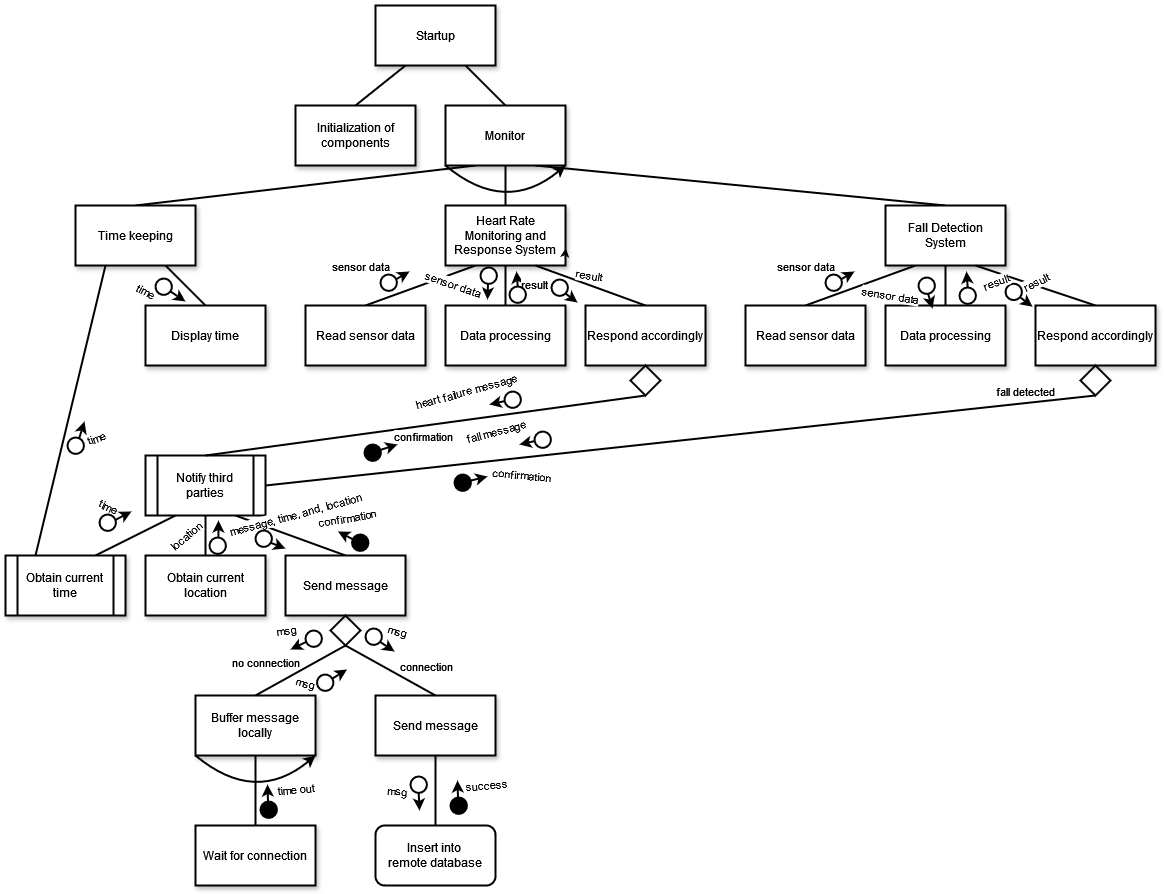
\includegraphics[width=\textwidth]{software-structure-chart.png}

\subsection{Heart Rate Monitor System}

The heart rate monitor system will as its name suggest, monitor heart rate, and seek for abnormalities in a heart rate pattern.
This module consist of three submodules: one for obtaining data, one for processing data, and one responding to accordingly to the data (notifying 3rd parties when abnormalities, otherwise no action required).
The data for this system will be obtained by reading a sensor.
Then, the system must analyse to data to determine whether a heart failure occurred.
Finally, depending on the result of the previous step, some action has to be taken.

\subsection{Fall Detection System}

The fall decection system consists of similar modules as the heart rate monitor system.
One for obtaining data by reading the gyroscope and accelerometer sensors.
Another module analyzes the obtained data and potentially performs some kind of processing on it, before determining whether a fall occurred.
Finally, a module that responds accordingly when a fall was detected by notifying a 3rd party, for example.

\subsection{Time Keeping}

The time keeping module is responsible for obtaining and displaying the current time on a display.

\subsection{Notify Third Parties}

When a fall occurred or abnormalities in the heart rate pattern were detected, a 3rd party has to be notified.
When there is no connection, the message has to be buffered and send later when the connection is restored.
When a connection is present, the message can and will immediately be send.
Together with this message, the current time and location will be send.

\subsection*{Language and Environment (If choosing ESP-IDF)}

The device will be developed using ESP-IDF.
ESP-IDF can be used in combination with VS Code, CLion, or any text editor, making it flexible for developers to use their preferred development workflow.
The ESP-IDF supports both language and library features of more recent \cpp{} standards, which is something the Arduino IDE lacks.
The ESP-IDF supports an Arduino component, making it possible to write code as would be done using the Arduino environment.

\subsection*{Language and Environment (If choosing Arduino IDE)}

The device will developed using the Arduino IDE.
The Arduino IDE is easy to setup, supports many microcontrollers, and there are many resources available for it.
All group members are already familiar with it, which makes it a time-efficient choice.

\subsection{Flowcharts}

Since the flowcharts of the heart rate monitor system and the fall detection system would look identical to each other, there is only made one to represent both of them.

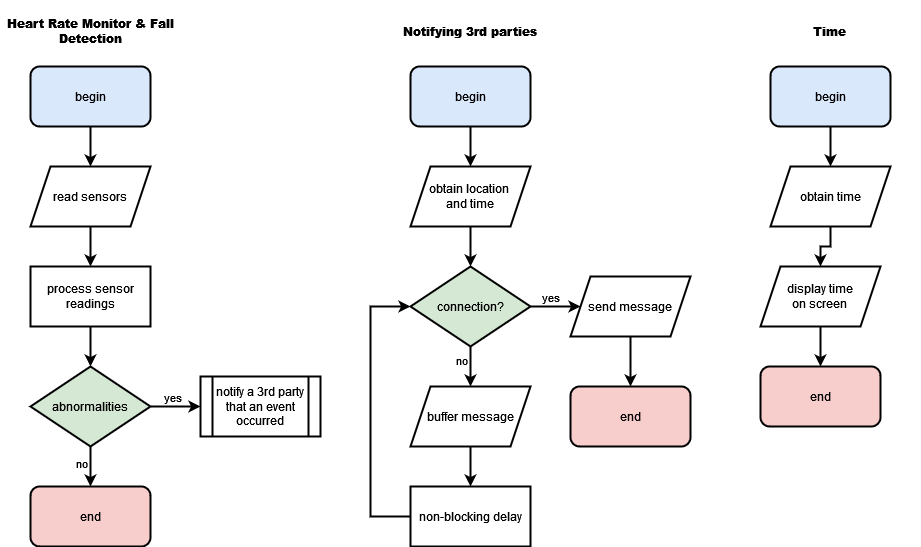
\includegraphics[width=\textwidth]{flowcharts.png}

\subsection{State Diagram}

\begin{tikzpicture}
    \node [state,initial,accepting] (1) {startup};
    \node [state,right of=1] (2) {monitoring};
    \node [state,below right of=2] (3) {fall detected};
    \node [state,above right of=2] (4) {heart failure}; 
    \node [state,align=center,below right of=4,right=0.1] (5) {try to notify\\a 3rd party};

    \draw (1) edge[above] node{} (2);
    \draw (2) edge[above,bend right,left=0.3] node{$detecting\:a\:fall$} (3);
    \draw (2) edge[above,bend  left,left=0.3] node{$detecting\:a\:heart\:failure$} (4);
    \draw (2) edge[above,bend  left,left=0.3] node{$detecting\:a\:heart\:failure$} (4);
    \draw (3) edge[bend right] node{} (5);
    \draw (4) edge[bend  left] node{} (5);
    \draw (5) edge[above,below=2] node{$message\:\:send$} (2);
    \draw (5) edge[loop right] node{$no\:connection$} (5);
\end{tikzpicture}

\noindent
When the device is turned on, it will initialize components in the startup state, after which it will transition to the monitor state.
In the monitor state, the device will display the time to a screen and wait for the detection of abnormalities.
Depending on what abnormality was detected, a transition to the "heart failure" state or "fall detected" state will occur.
After the detection of such event, 3rd parties need to be notified.
If the device is not able to establish a connection, it needs to buffer the message and try again later.
If the device did achieve to establish a connection, it will send a message and transition back to the monitor state.

\clearpage


\bibliographystyle{apacite}
%\bibliographystyle{IEEEtranN}
\bibliography{research}

\end{document}

